\section{Approximate Nearest Neighbors Oh Yeah (Annoy)}

\subsection{Introduction to Annoy}

Approximate Nearest Neighbors Oh Yeah (Annoy) is a tree-based approach for approximate nearest neighbor (ANN) search. It was developed by Bernhardsson during Spotify's Hack Week in 2013 \cite{spotify-annoy} for music recommendation.

An Annoy tree is constructed using random projections: at each intermediate node, a hyperplane is defined by sampling two points from the subset and placing it equidistant from them, thereby dividing the space into two subspaces. The recursive process continues until a single tree is formed \cite{spotify-annoy}.

Although Annoy does not provide formal theoretical guarantees like LSH or HNSW, it has demonstrated good empirical performance. By offering a favorable trade-off between query speed, memory usage, and accuracy \cite{Li-Zhang-Sun-Wang-Zhang-Lin-2016}, it is often used in practice and is also referenced in research on approximate nearest neighbor search.

The Annoy implementation is available at GitHub\footnote{\url{https://github.com/spotify/annoy}}.

\subsection{Description of Annoy}

The description provided in this section is based on the official Spotify Annoy repository \cite{spotify-annoy} and Bernhardsson's presentation on Annoy \cite{erikbern-ann-presentation}.

\subsubsection{Indexing: Tree}

\noindent
To illustrate the construction of an Annoy index, a set of points representing vectors in the space is shown (Figure~\ref{fig:annoy-1}). For visualization purposes, a 2-dimensional example is used; in practice, vectors typically reside in much higher-dimensional spaces.

\begin{figure}[H]
    \centering
    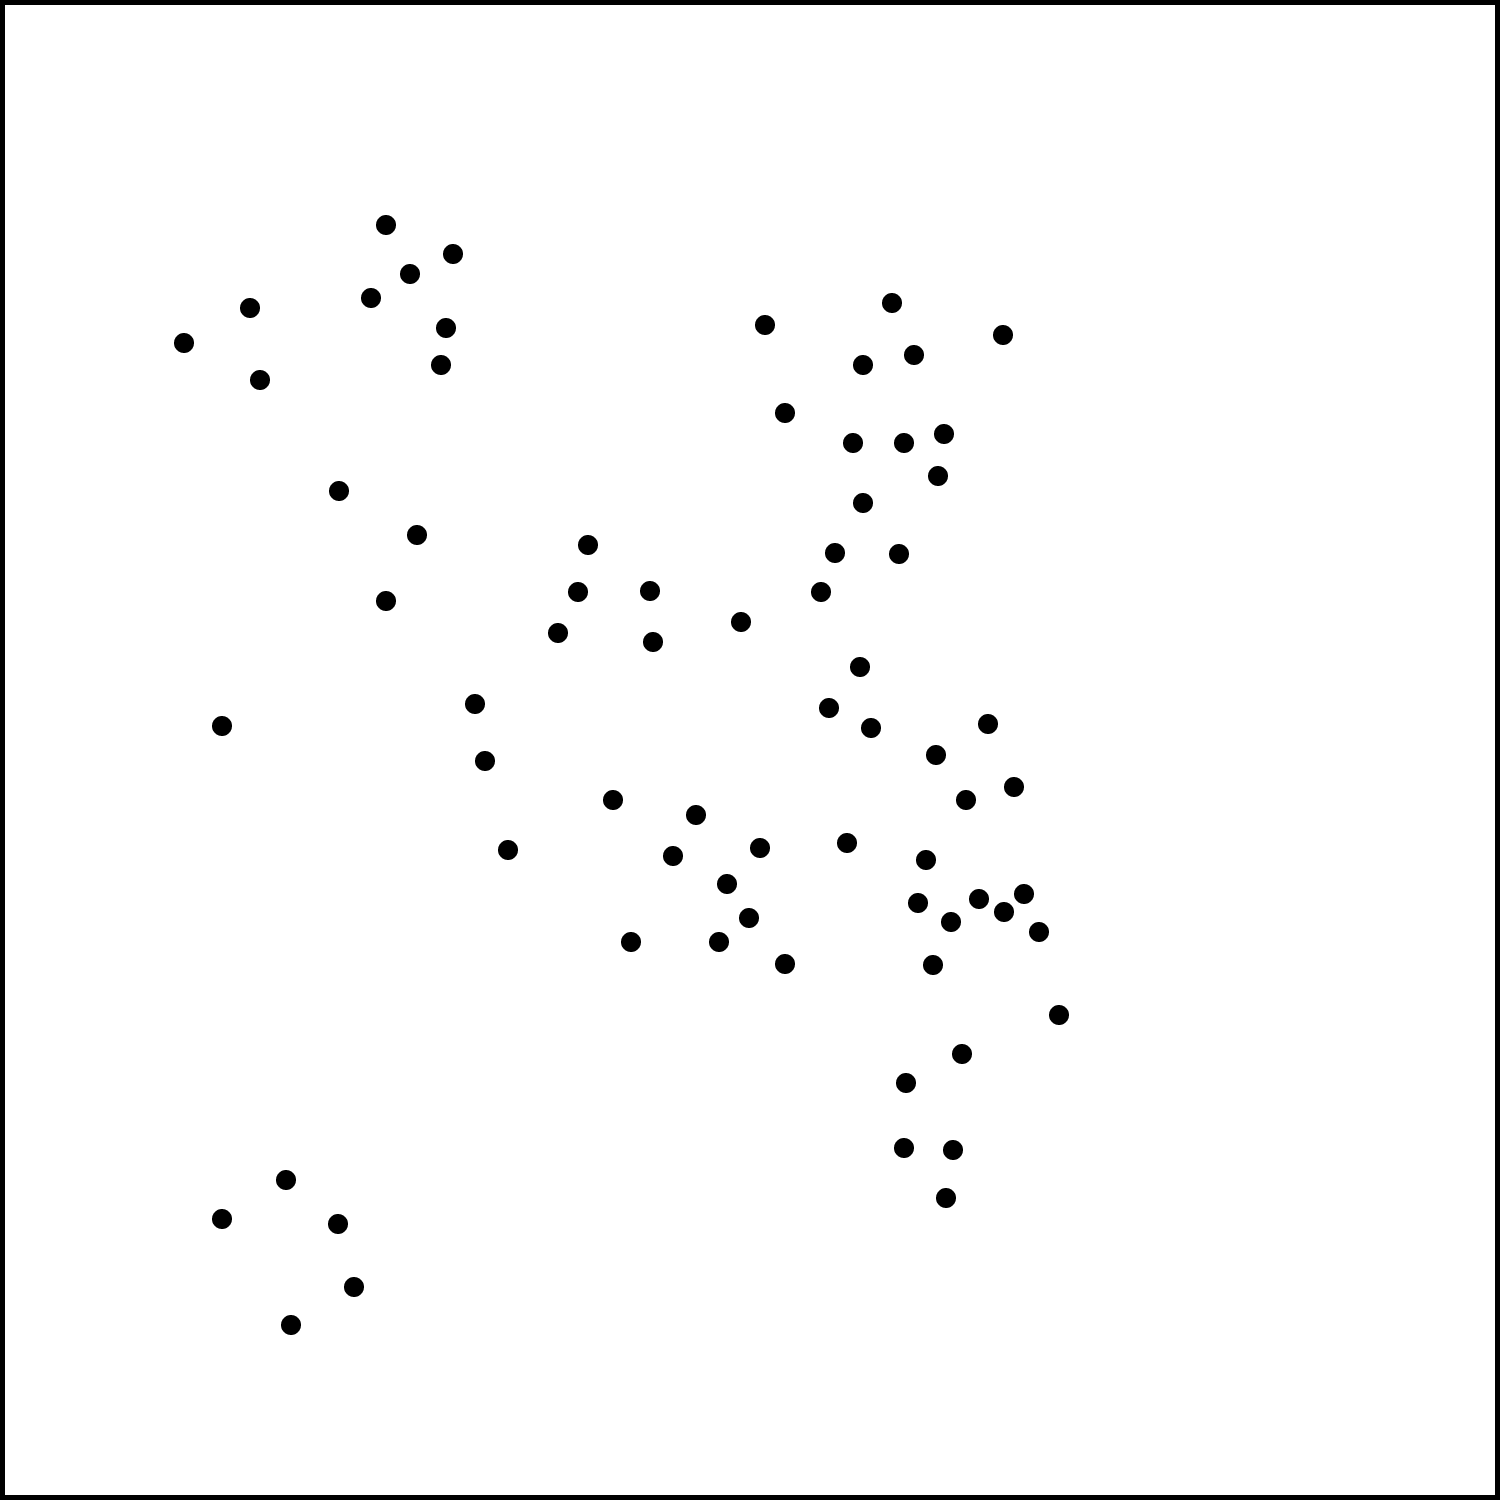
\includegraphics[width=0.48\textwidth]{chapters/algorithms/annoy/figures/points.png}
    \caption{Initial set of points in 2D space.}
    \label{fig:annoy-1}
\end{figure}

\newpage

\noindent
The goal is to construct a data structure that allows nearest neighbor queries to be answered in sublinear time. To support this, Annoy builds a binary tree in which each node represents a random partition of the space. The process begins with a single split of the space (Figure~\ref{fig:annoy-2-a}).

Each split is performed by randomly selecting two points and constructing a hyperplane equidistant from them. This hyperplane divides the current subspace into two halves, with each half assigned to a child node in the binary tree. The partitioning continues recursively for each resulting subspace (Figure~\ref{fig:annoy-2-b}). In practice, the hyperplane itself does not need to be explicitly computed; each vector is assigned to a side based on which of the two selected points it is closer to.

\begin{figure}[H]
    \centering
    \begin{subfigure}[t]{0.48\textwidth}
        \centering
        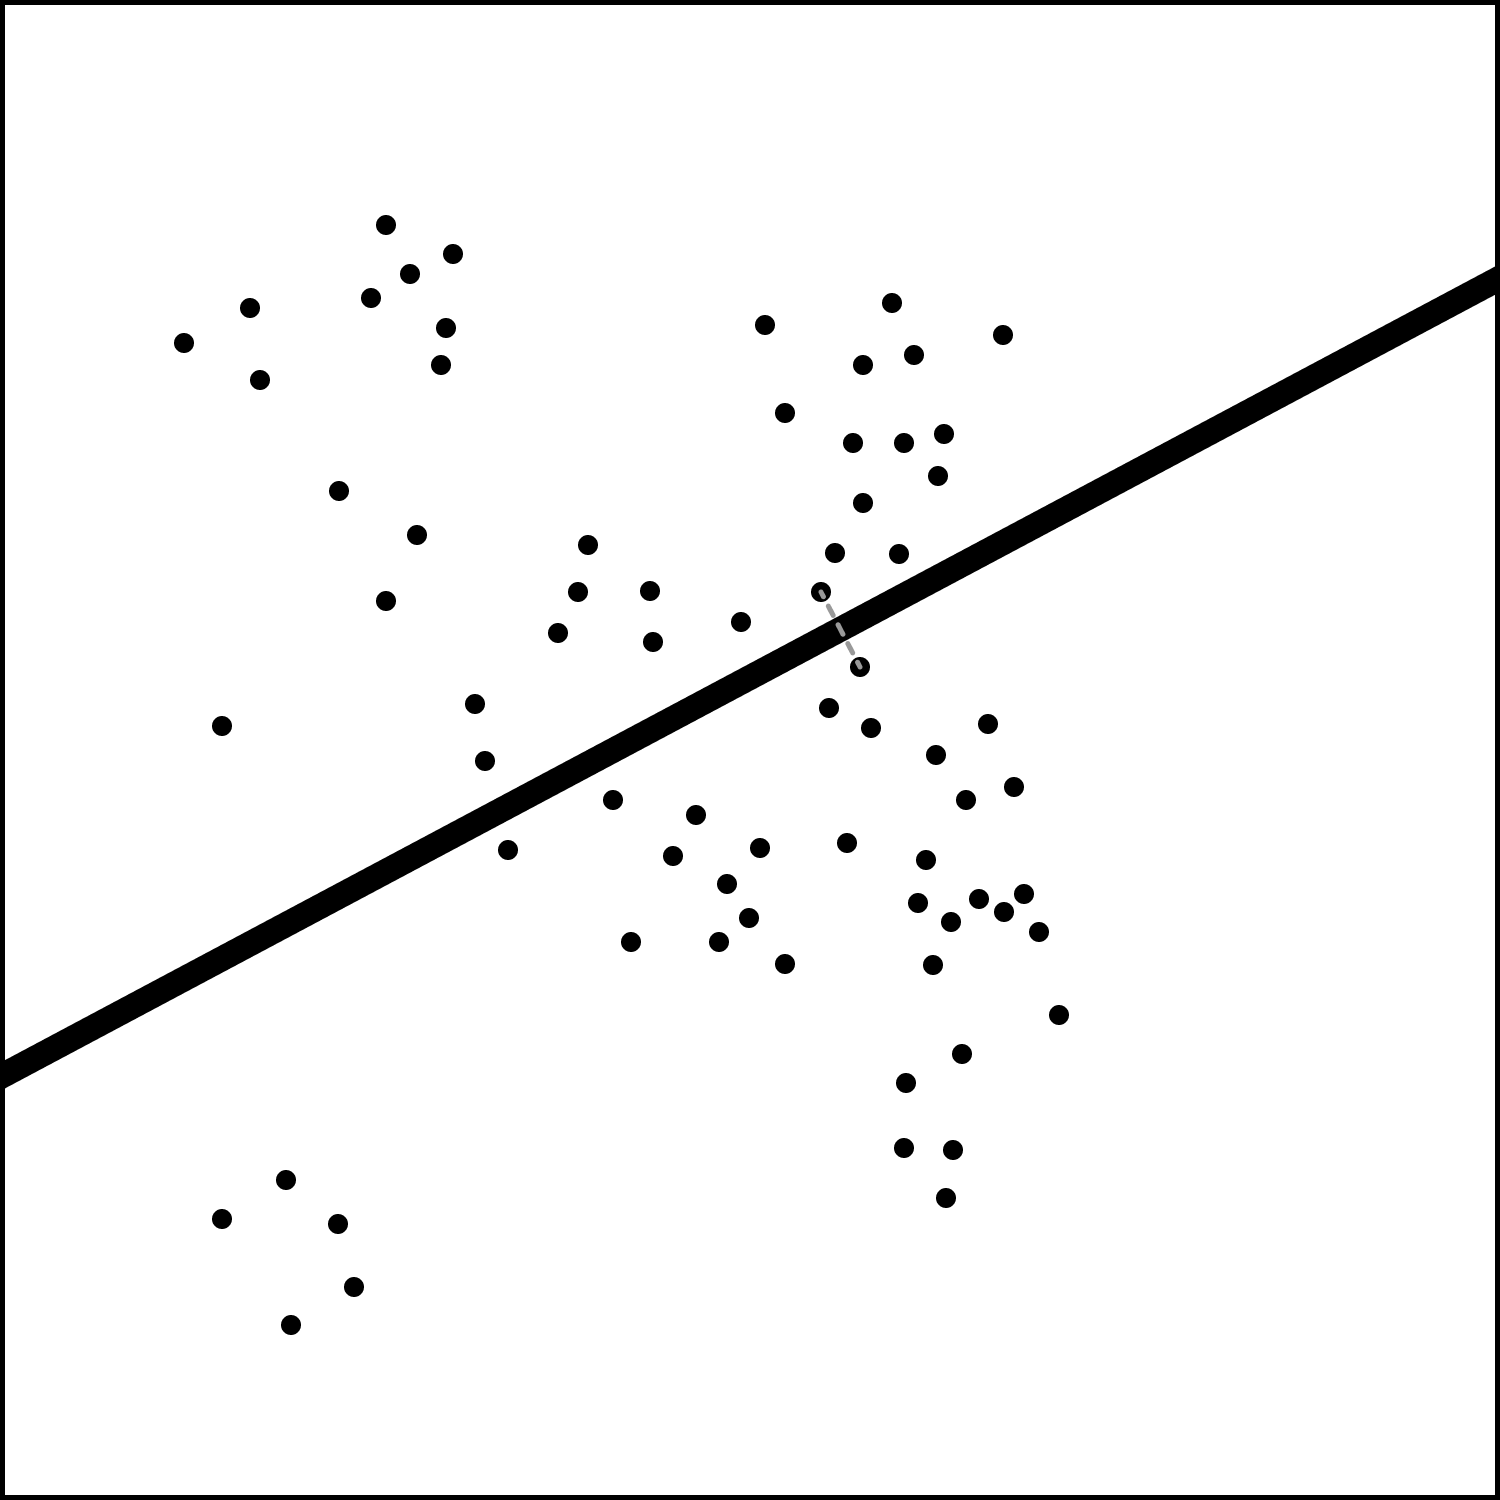
\includegraphics[width=\textwidth]{chapters/algorithms/annoy/figures/initial-split.png}
        \caption{Initial split of the space using a hyperplane.}
        \label{fig:annoy-2-a}
    \end{subfigure}
    \hfill
    \begin{subfigure}[t]{0.48\textwidth}
        \centering
        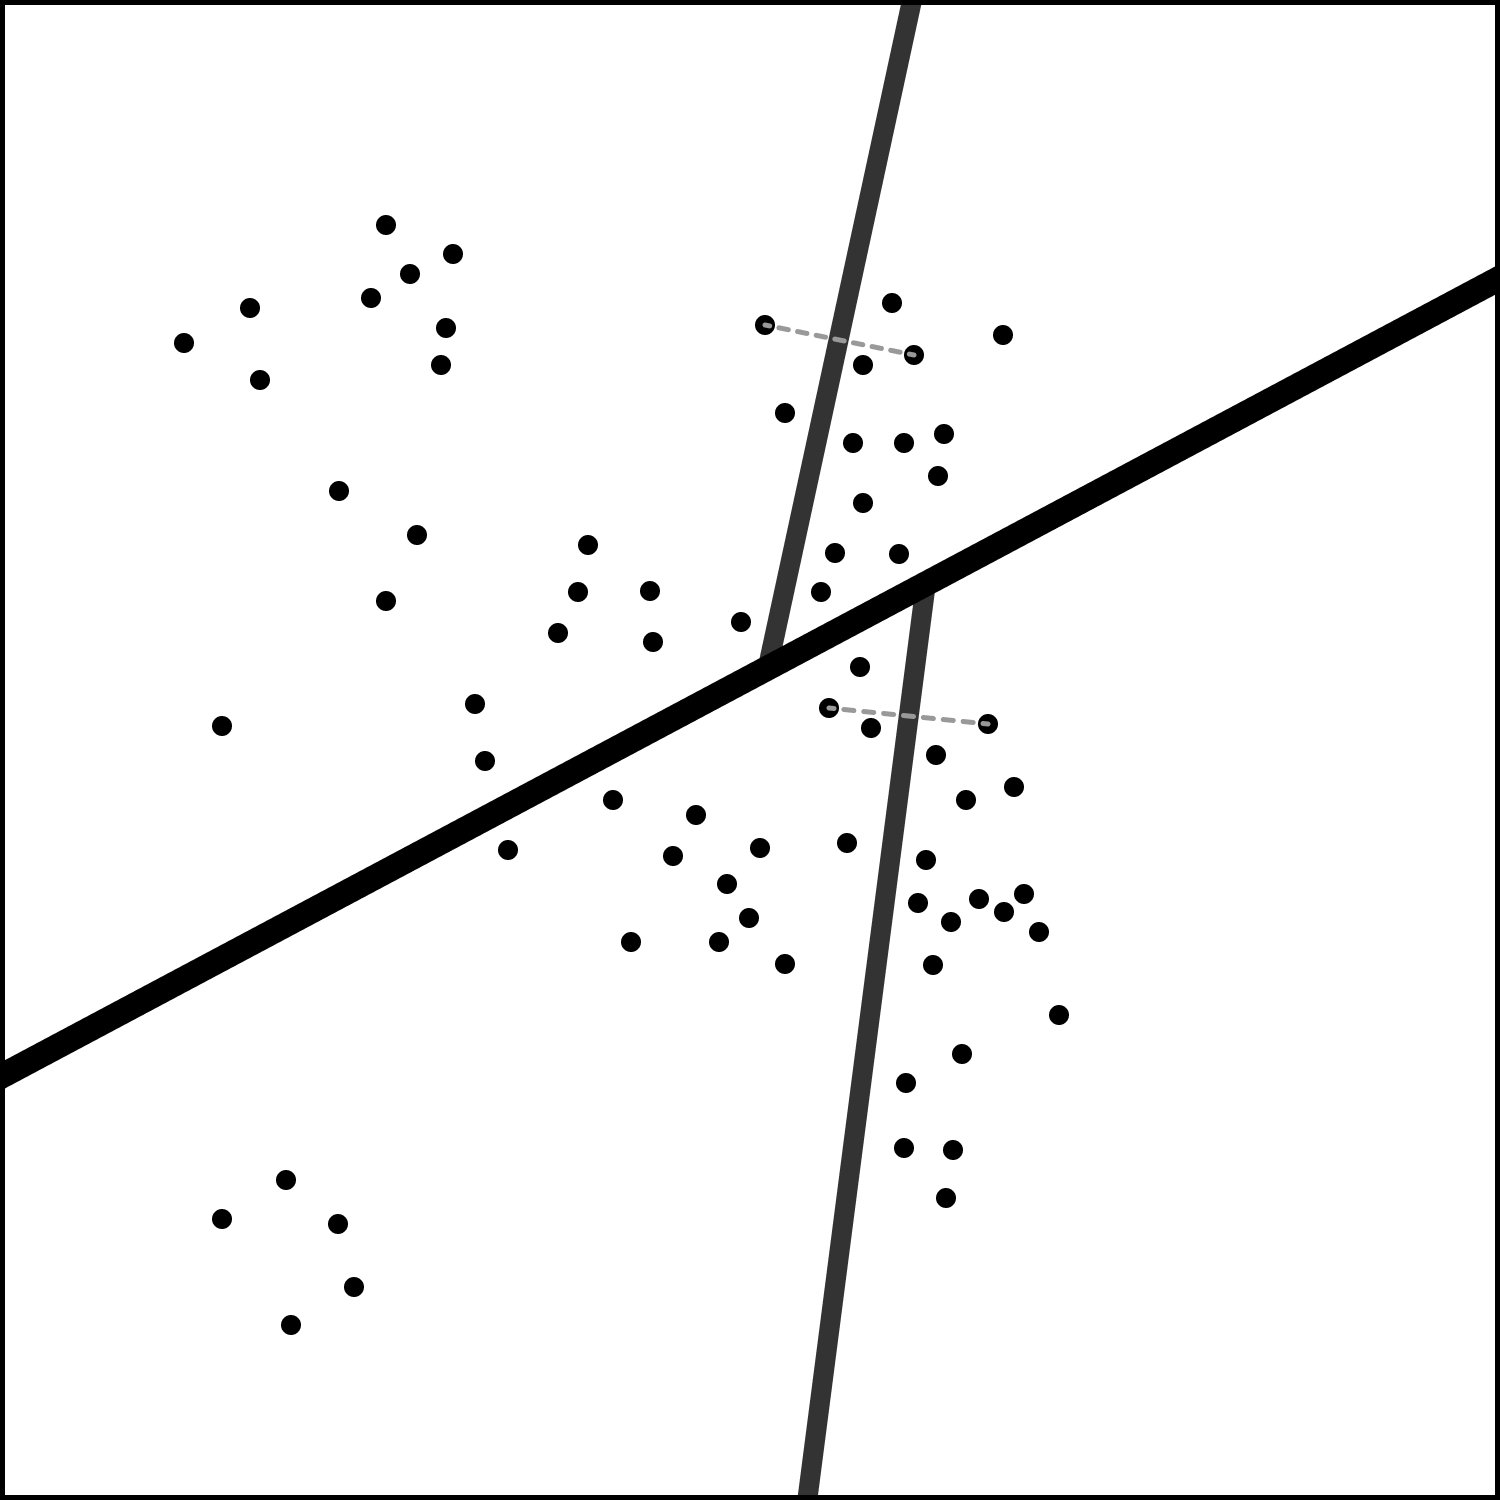
\includegraphics[width=\textwidth]{chapters/algorithms/annoy/figures/recursive-splits.png}
        \caption{Recursive splits of subspaces.}
        \label{fig:annoy-2-b}
    \end{subfigure}
    \caption{Initial and recursive splits in the construction of an Annoy tree.}
    \label{fig:annoy-2}
\end{figure}

\noindent
The recursive partitioning proceeds until each leaf node contains at most $K$ points (Figure~\ref{fig:annoy-3}).

\begin{figure}[H]
    \centering
    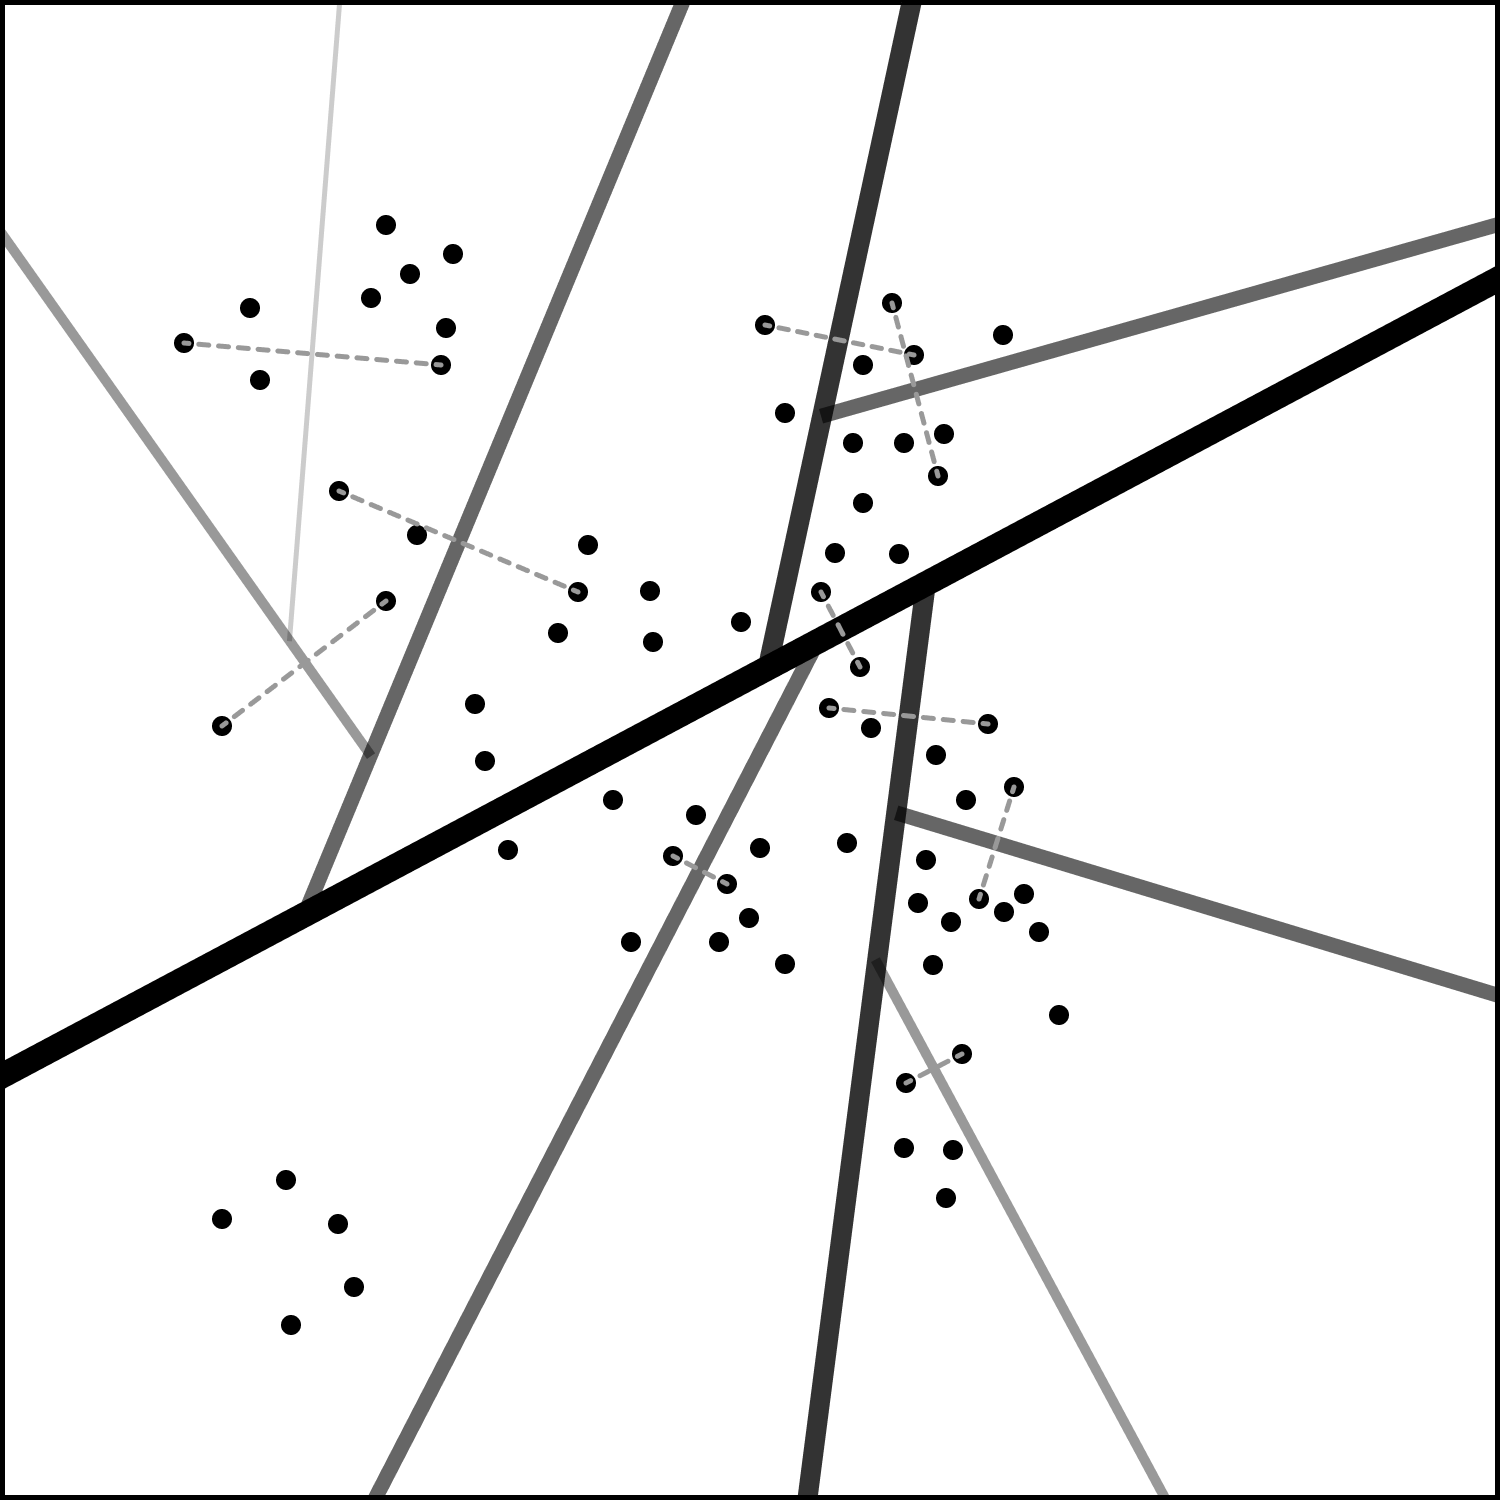
\includegraphics[width=0.48\textwidth]{chapters/algorithms/annoy/figures/final-splits.png}
    \caption{Final partitions of the space with a maximum of $K = 10$ points per leaf.}
    \label{fig:annoy-3}
\end{figure}

\noindent
The structure of the binary tree (Figure~\ref{fig:annoy-4}) reflects the hierarchical partitioning of the space. Each leaf node in the tree corresponds to one of the final subspaces.

\begin{figure}[H]
    \centering
    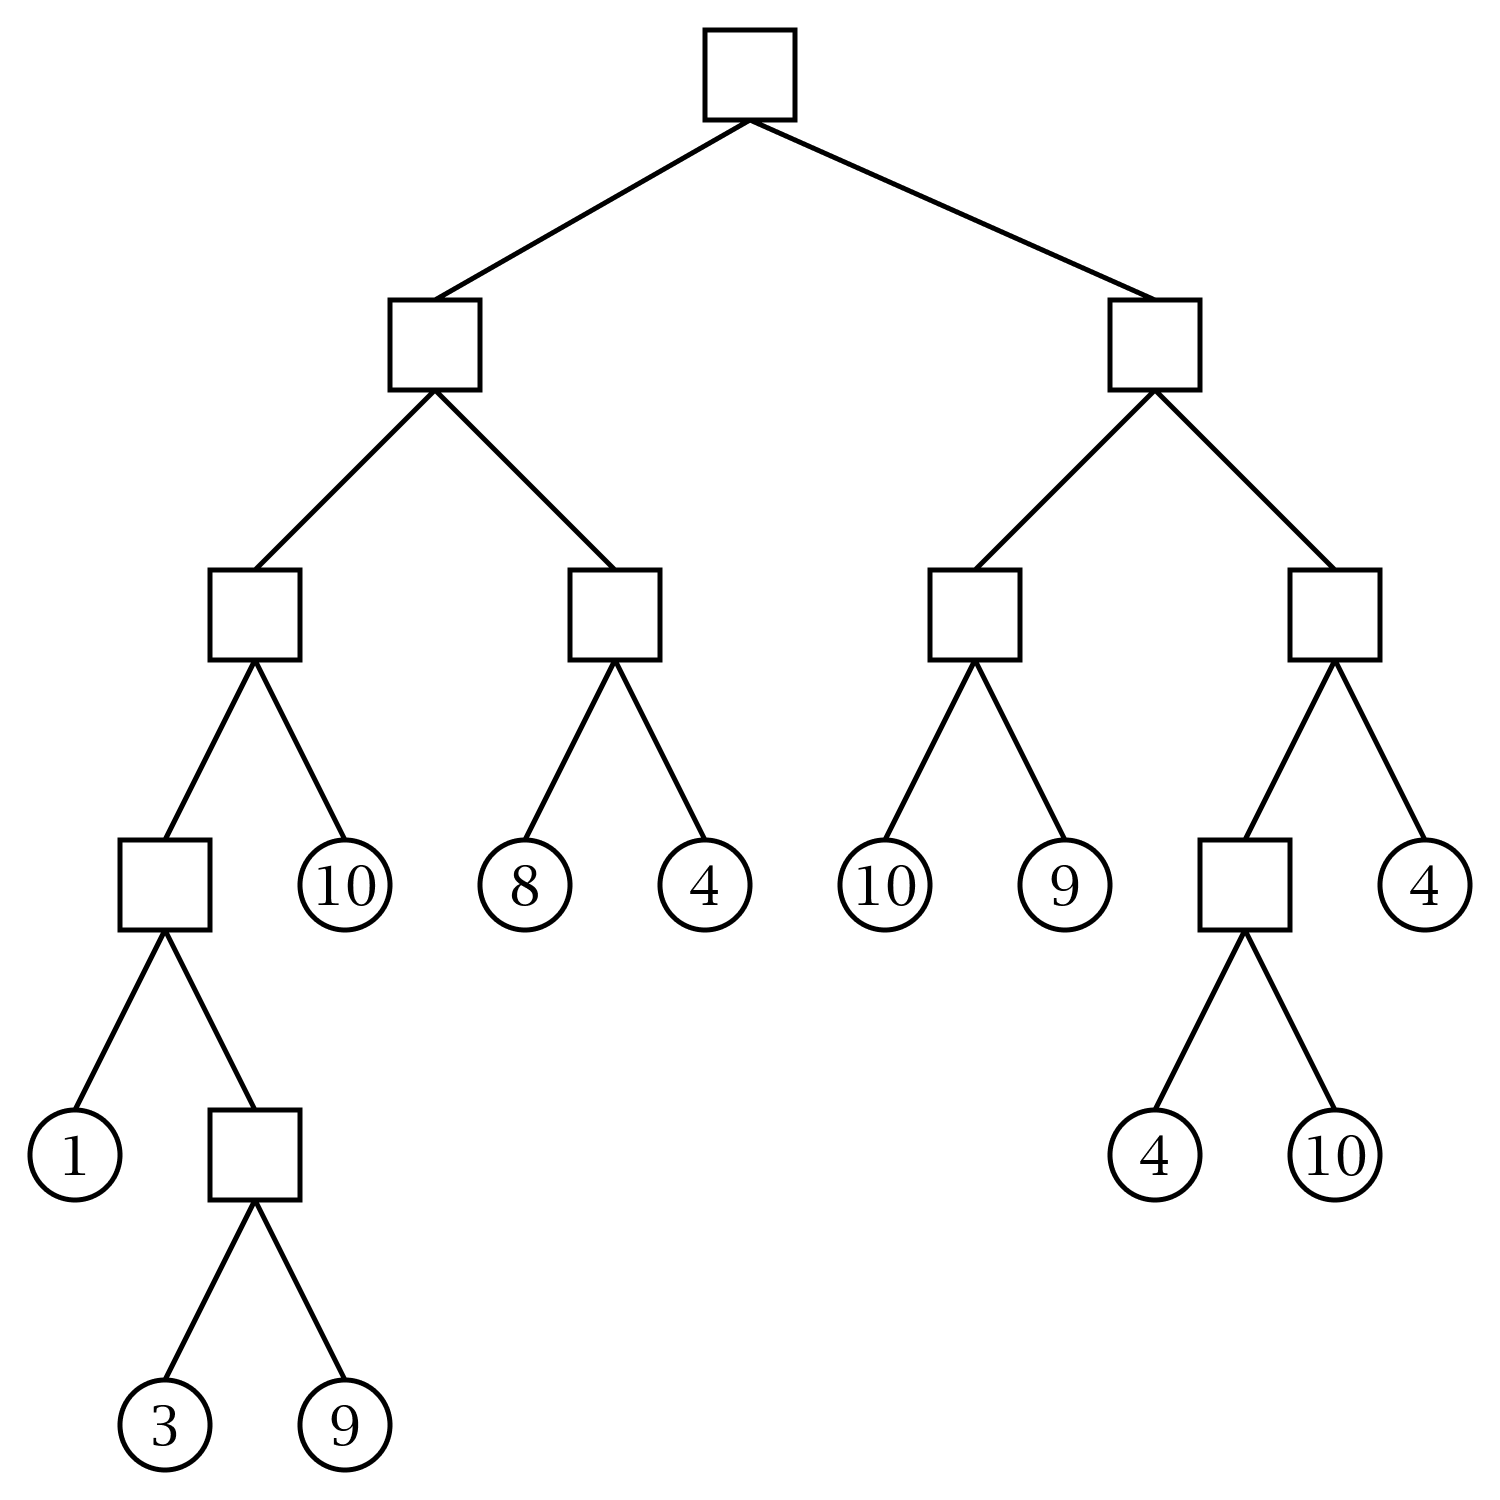
\includegraphics[width=0.48\textwidth]{chapters/algorithms/annoy/figures/tree-1.png}
    \caption{Binary tree corresponding to the final partitioning of the space.}
    \label{fig:annoy-4}
\end{figure}

\noindent
Points that are close to each other are likely to remain within the same or neighboring leaf nodes. Consequently, hyperplanes rarely separate points that are near each other, preserving local proximity within the tree structure.

\subsubsection{Querying}

\noindent
Once the space has been partitioned, a query point is evaluated within the structure to search for its nearest neighbors (Figure~\ref{fig:annoy-5}).

\begin{figure}[H]
    \centering
    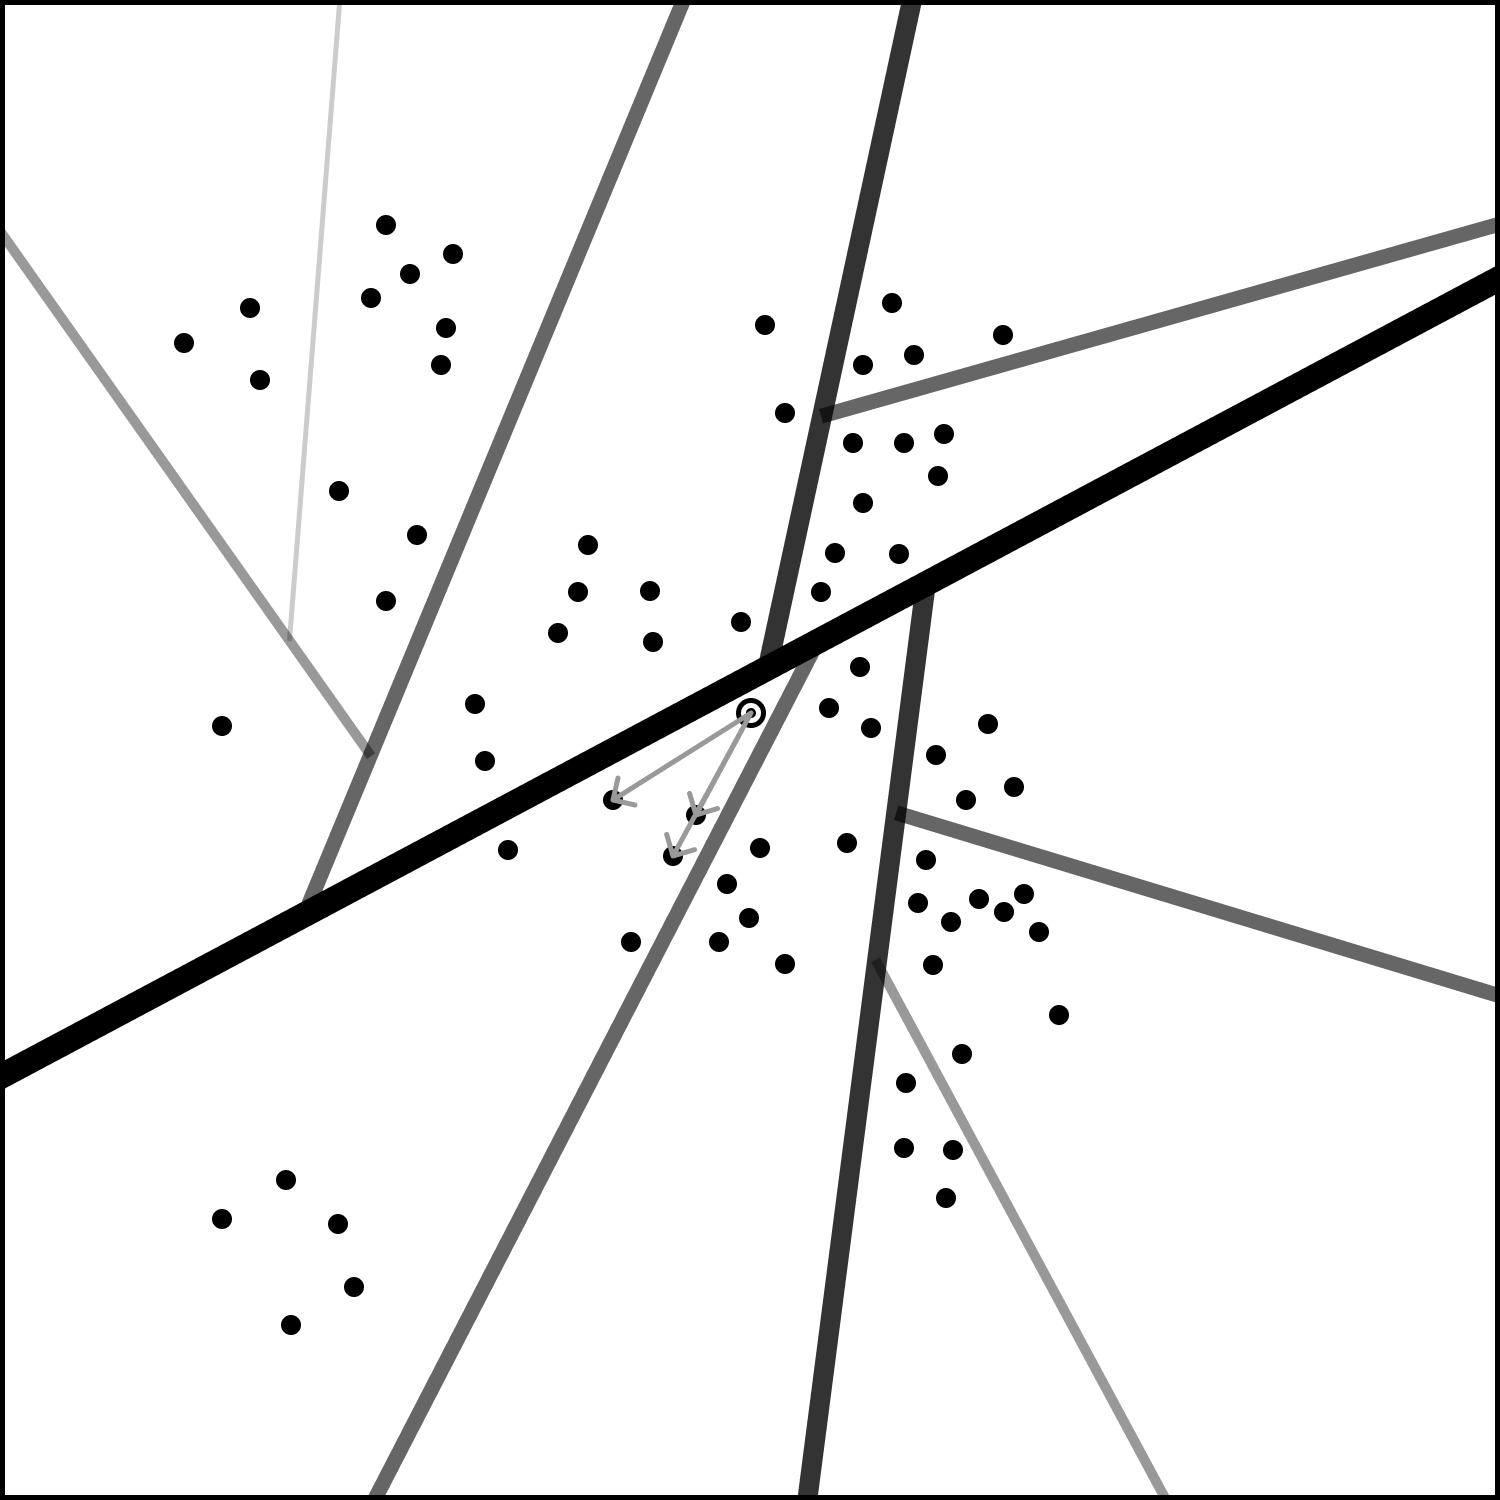
\includegraphics[width=0.48\textwidth]{chapters/algorithms/annoy/figures/query-1.png}
    \caption{Query point within the partitioned space.}
    \label{fig:annoy-5}
\end{figure}

\newpage

\noindent
To perform a query in the structure, the binary tree is traversed from the root (Figure~\ref{fig:annoy-6}). At each step, the query point is assigned to one of the two child nodes depending on which side of the hyperplane it lies. This decision can be made by comparing the distances from the query vector to the two reference vectors used to define the split. Since the height of the tree is logarithmic in the number of points, the traversal can be completed in logarithmic time complexity.

\begin{figure}[H]
    \centering
    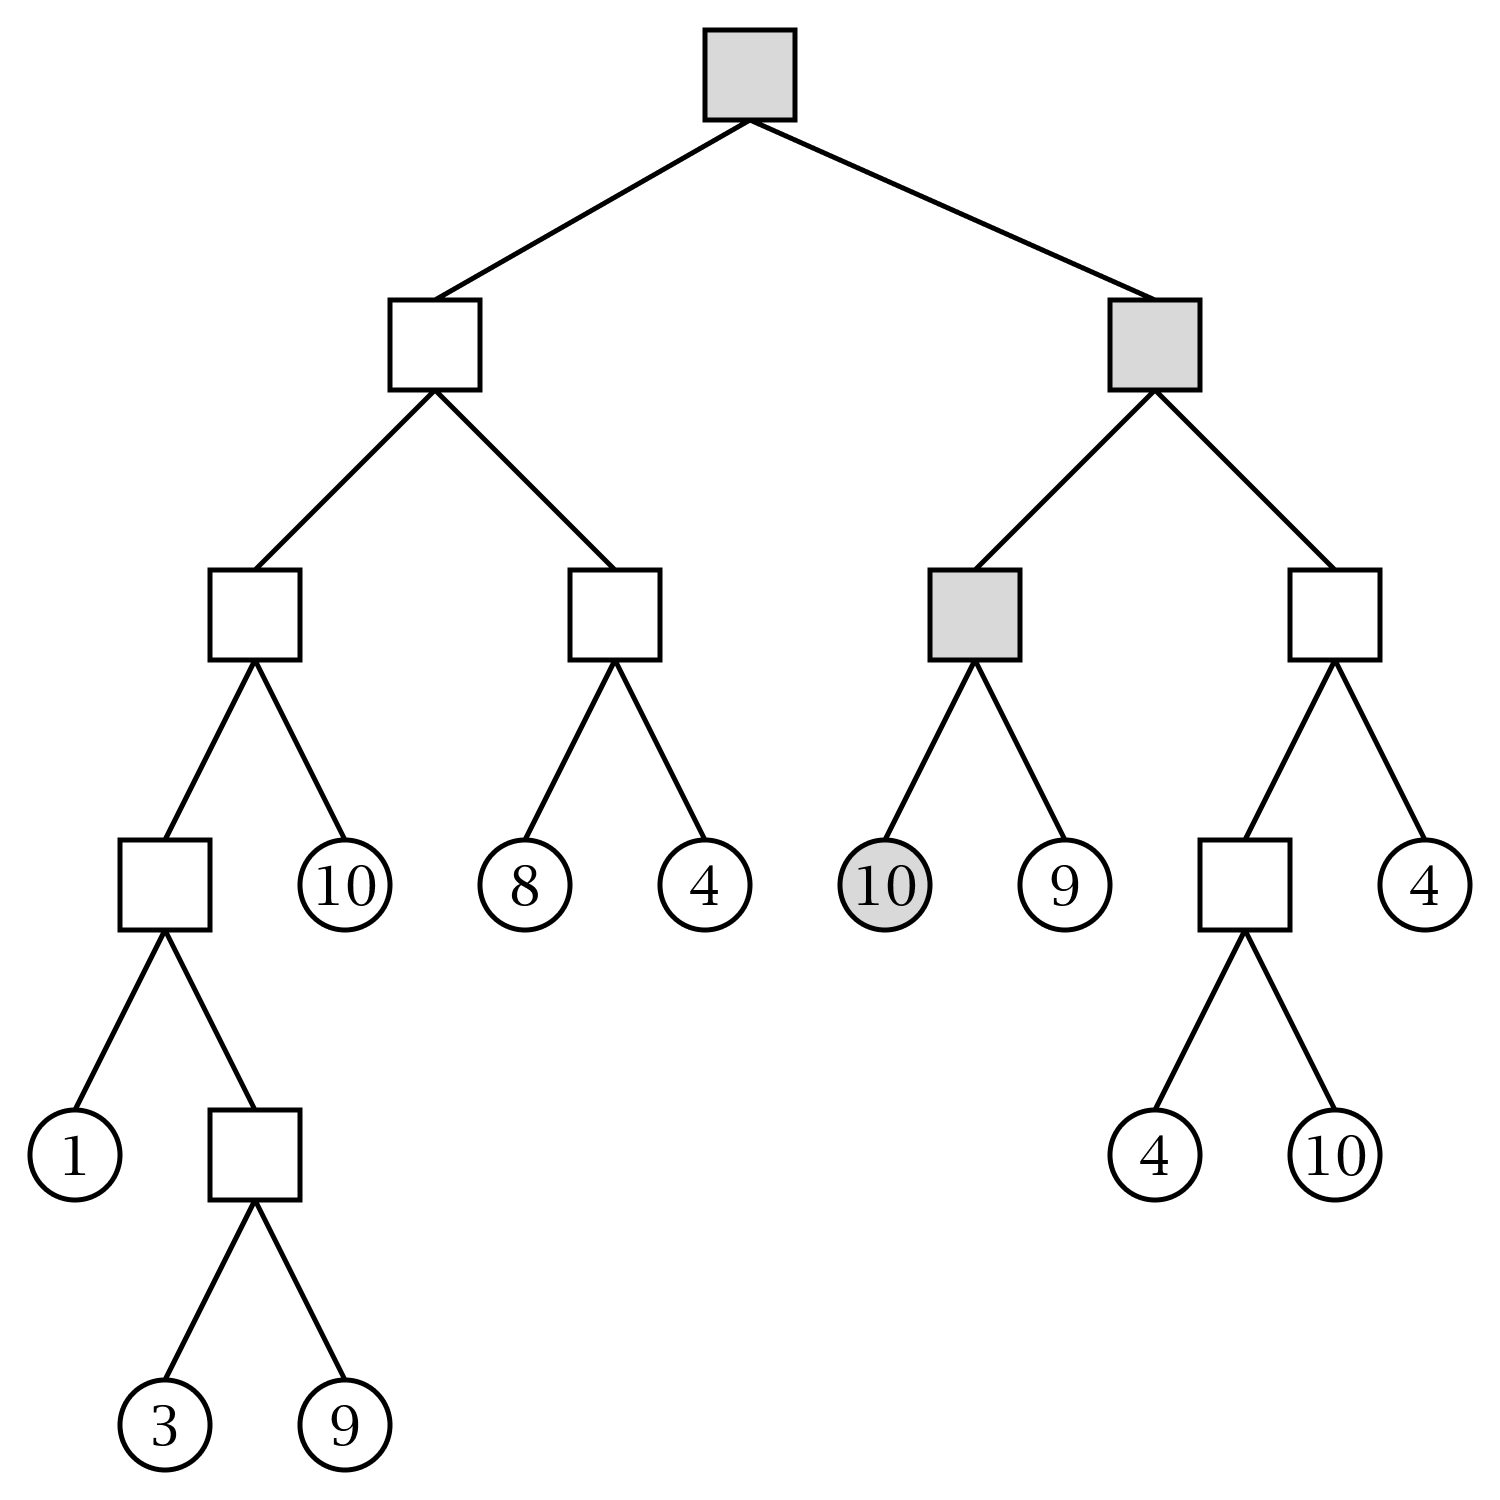
\includegraphics[width=0.48\textwidth]{chapters/algorithms/annoy/figures/traversal-1.png}
    \caption{Traversal path in the binary tree for the query point.}
    \label{fig:annoy-6}
\end{figure}

\noindent
This procedure, however, has two limitations. First, the number of neighbors retrieved is bounded by the capacity of the leaf node, which may be smaller than the desired number of nearest neighbors. Second, some true nearest neighbors may reside outside the leaf region reached by the query, leading to reduced accuracy.

\subsubsection{Indexing: Forest}

\noindent
To mitigate the limitations of individual trees and enhance search accuracy, multiple trees are constructed to form a forest (Figure~\ref{fig:annoy-7}). Each tree is generated independently using a different random set of splits, and a query is evaluated across all trees simultaneously.

\begin{figure}[H]
    \centering
    \begin{subfigure}[t]{0.48\textwidth}
        \centering
        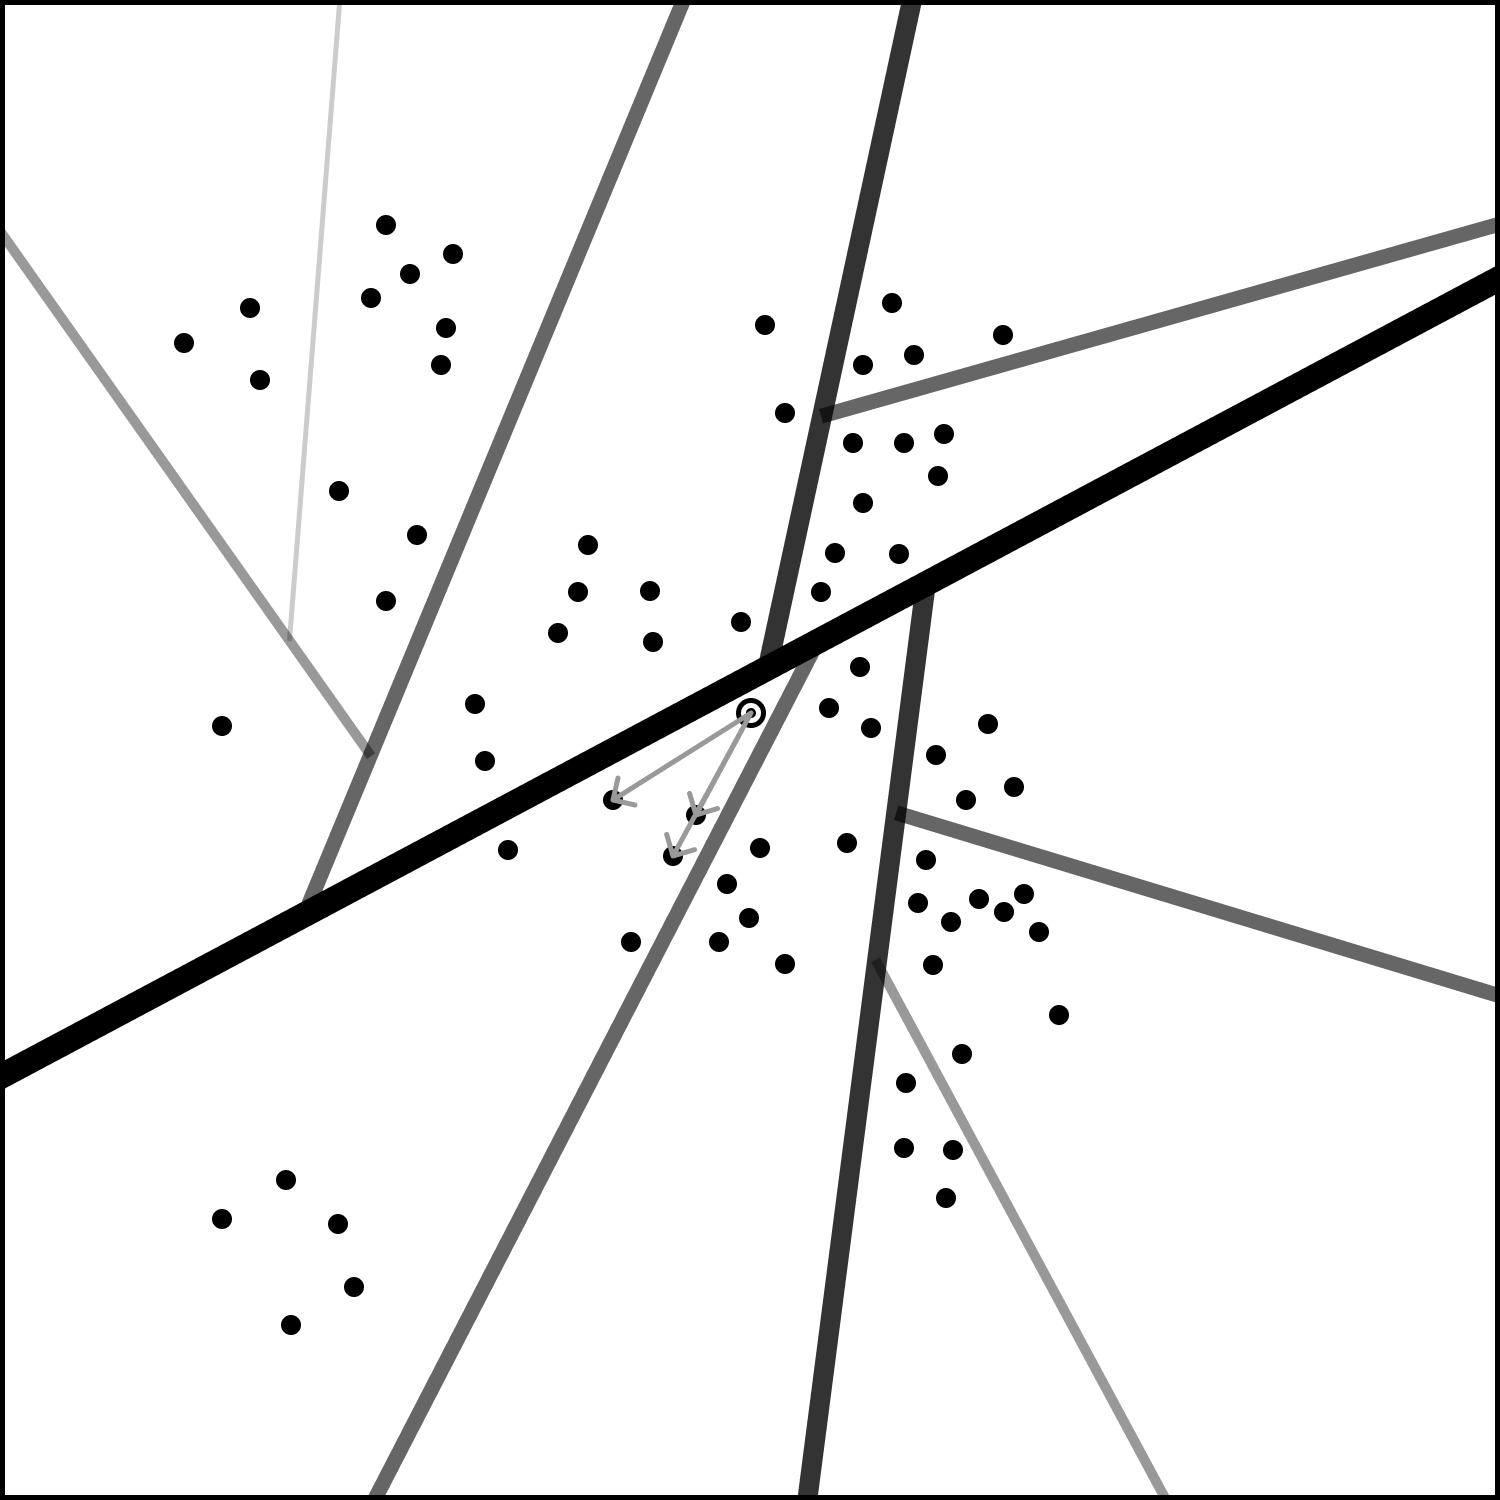
\includegraphics[width=\textwidth]{chapters/algorithms/annoy/figures/query-1.png}
        \caption{Final partitioning of the first tree.}
        \label{fig:annoy-7-a}
    \end{subfigure}
    \hfill
    \begin{subfigure}[t]{0.48\textwidth}
        \centering
        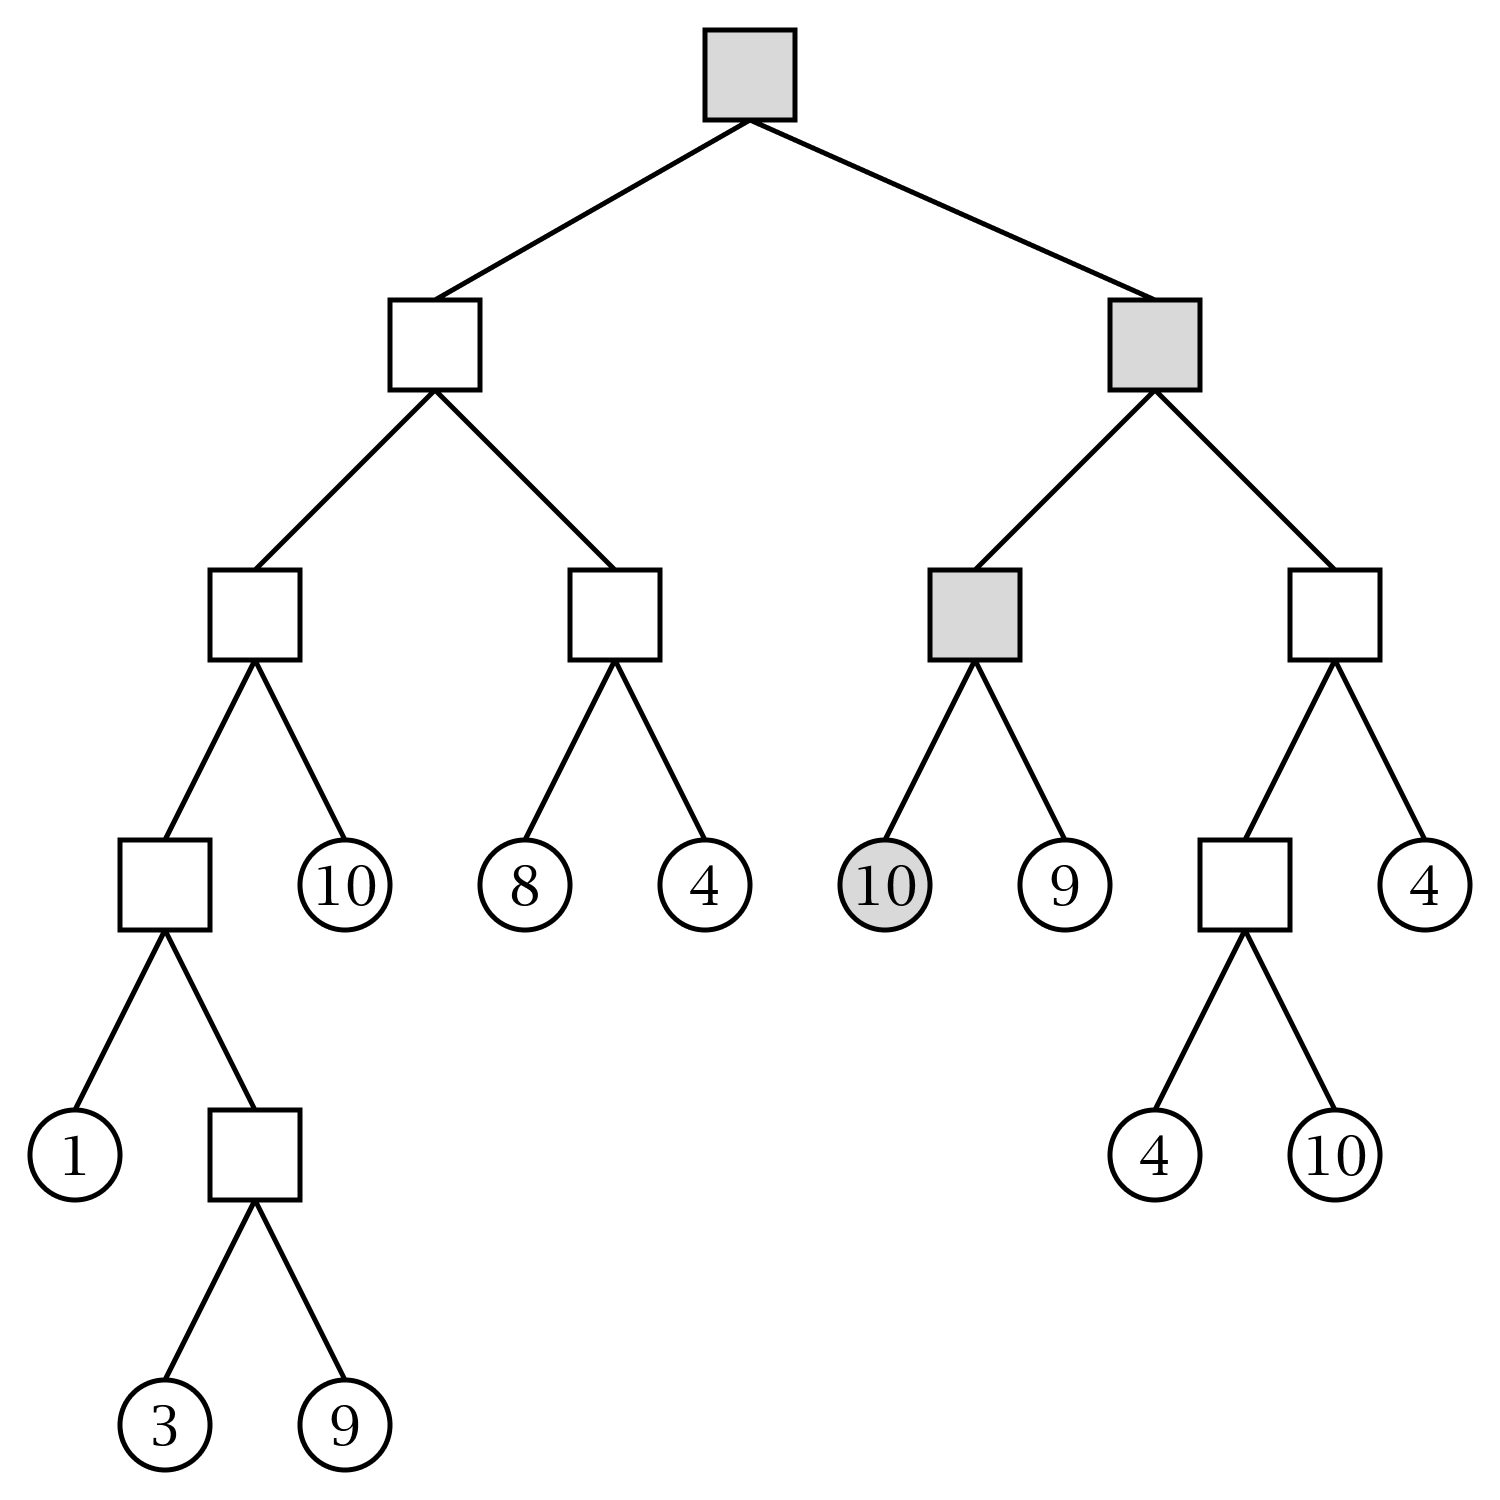
\includegraphics[width=\textwidth]{chapters/algorithms/annoy/figures/traversal-1.png}
        \caption{Binary tree corresponding to the first partitioning.}
        \label{fig:annoy-7-b}
    \end{subfigure}
    
    \vskip 0.3cm
    
    \begin{subfigure}[t]{0.48\textwidth}
        \centering
        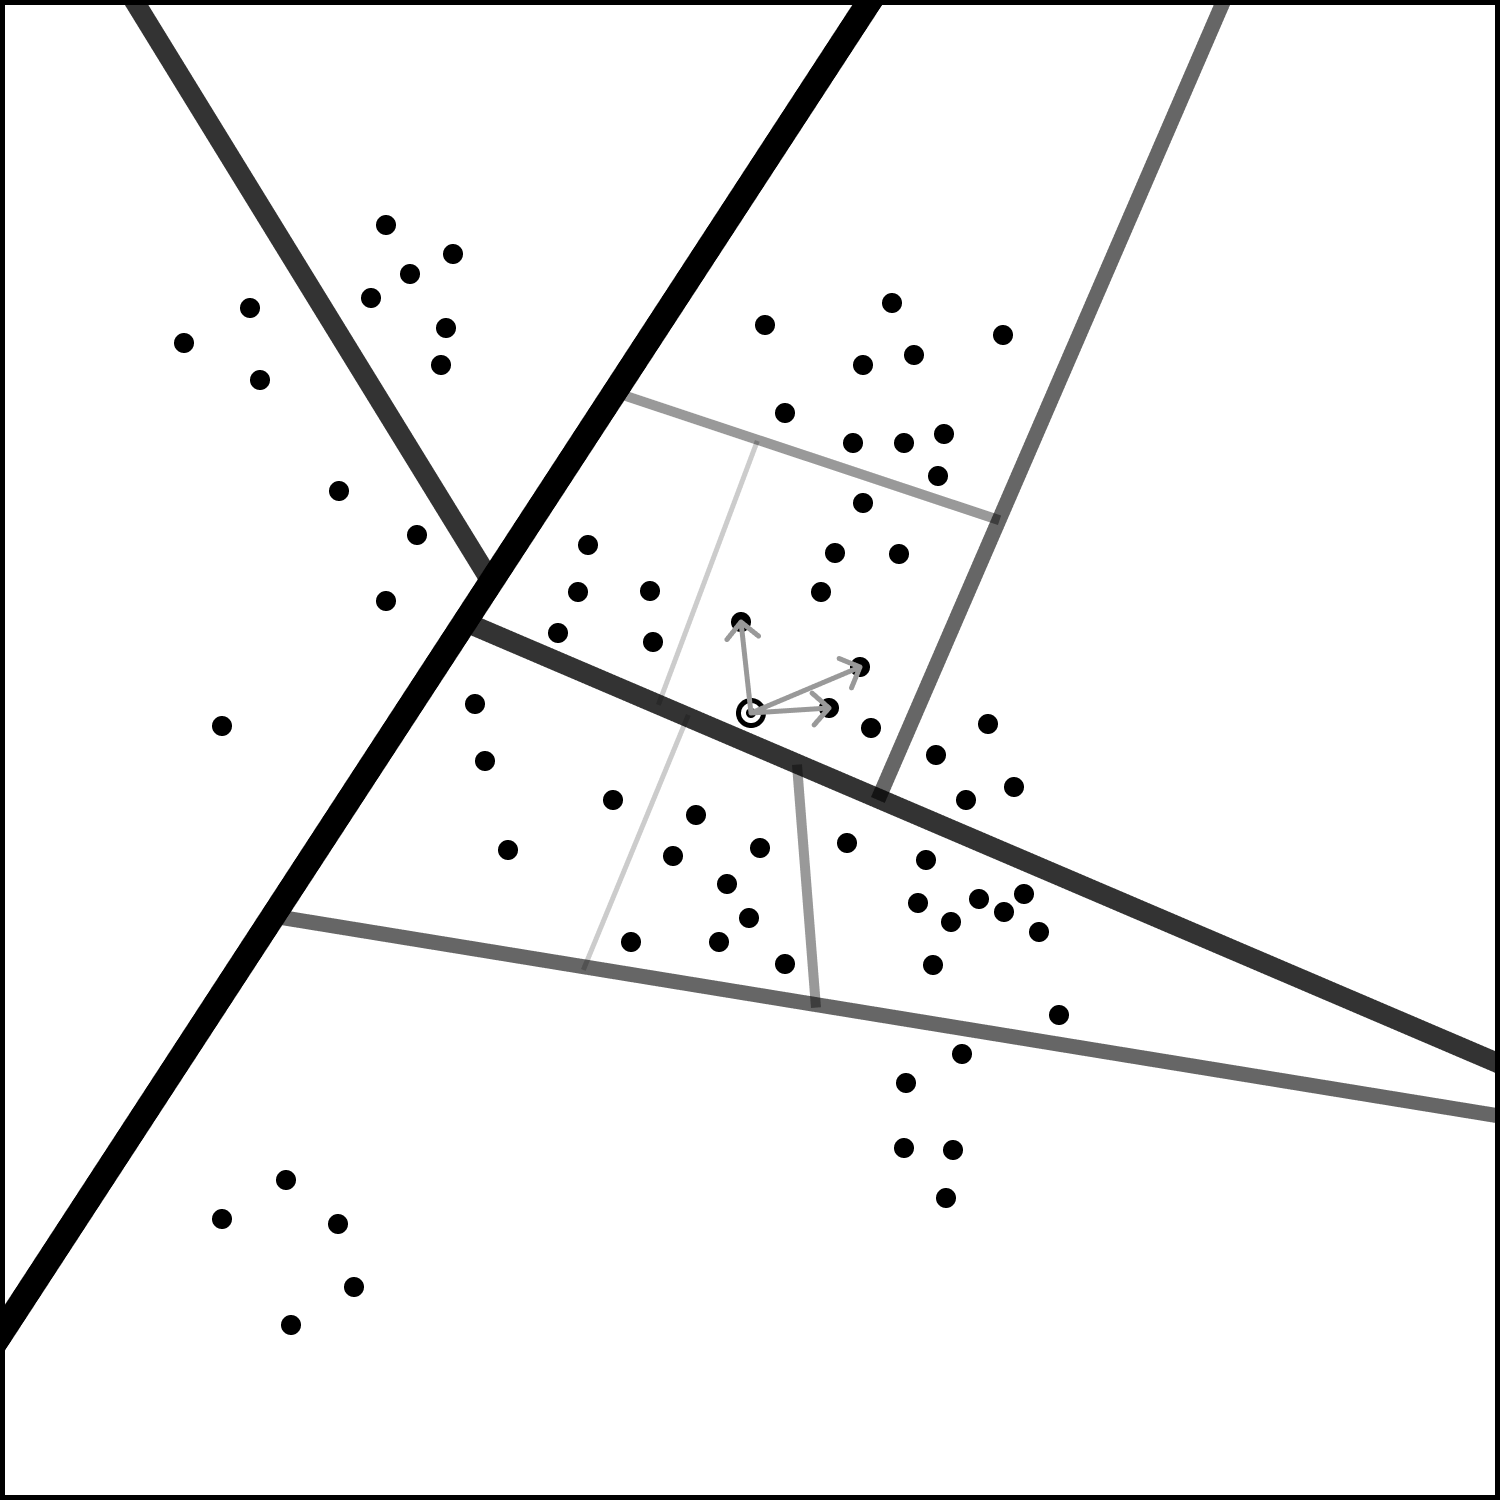
\includegraphics[width=\textwidth]{chapters/algorithms/annoy/figures/query-2.png}
        \caption{Final partitioning of the second tree.}
        \label{fig:annoy-7-c}
    \end{subfigure}
    \hfill
    \begin{subfigure}[t]{0.48\textwidth}
        \centering
        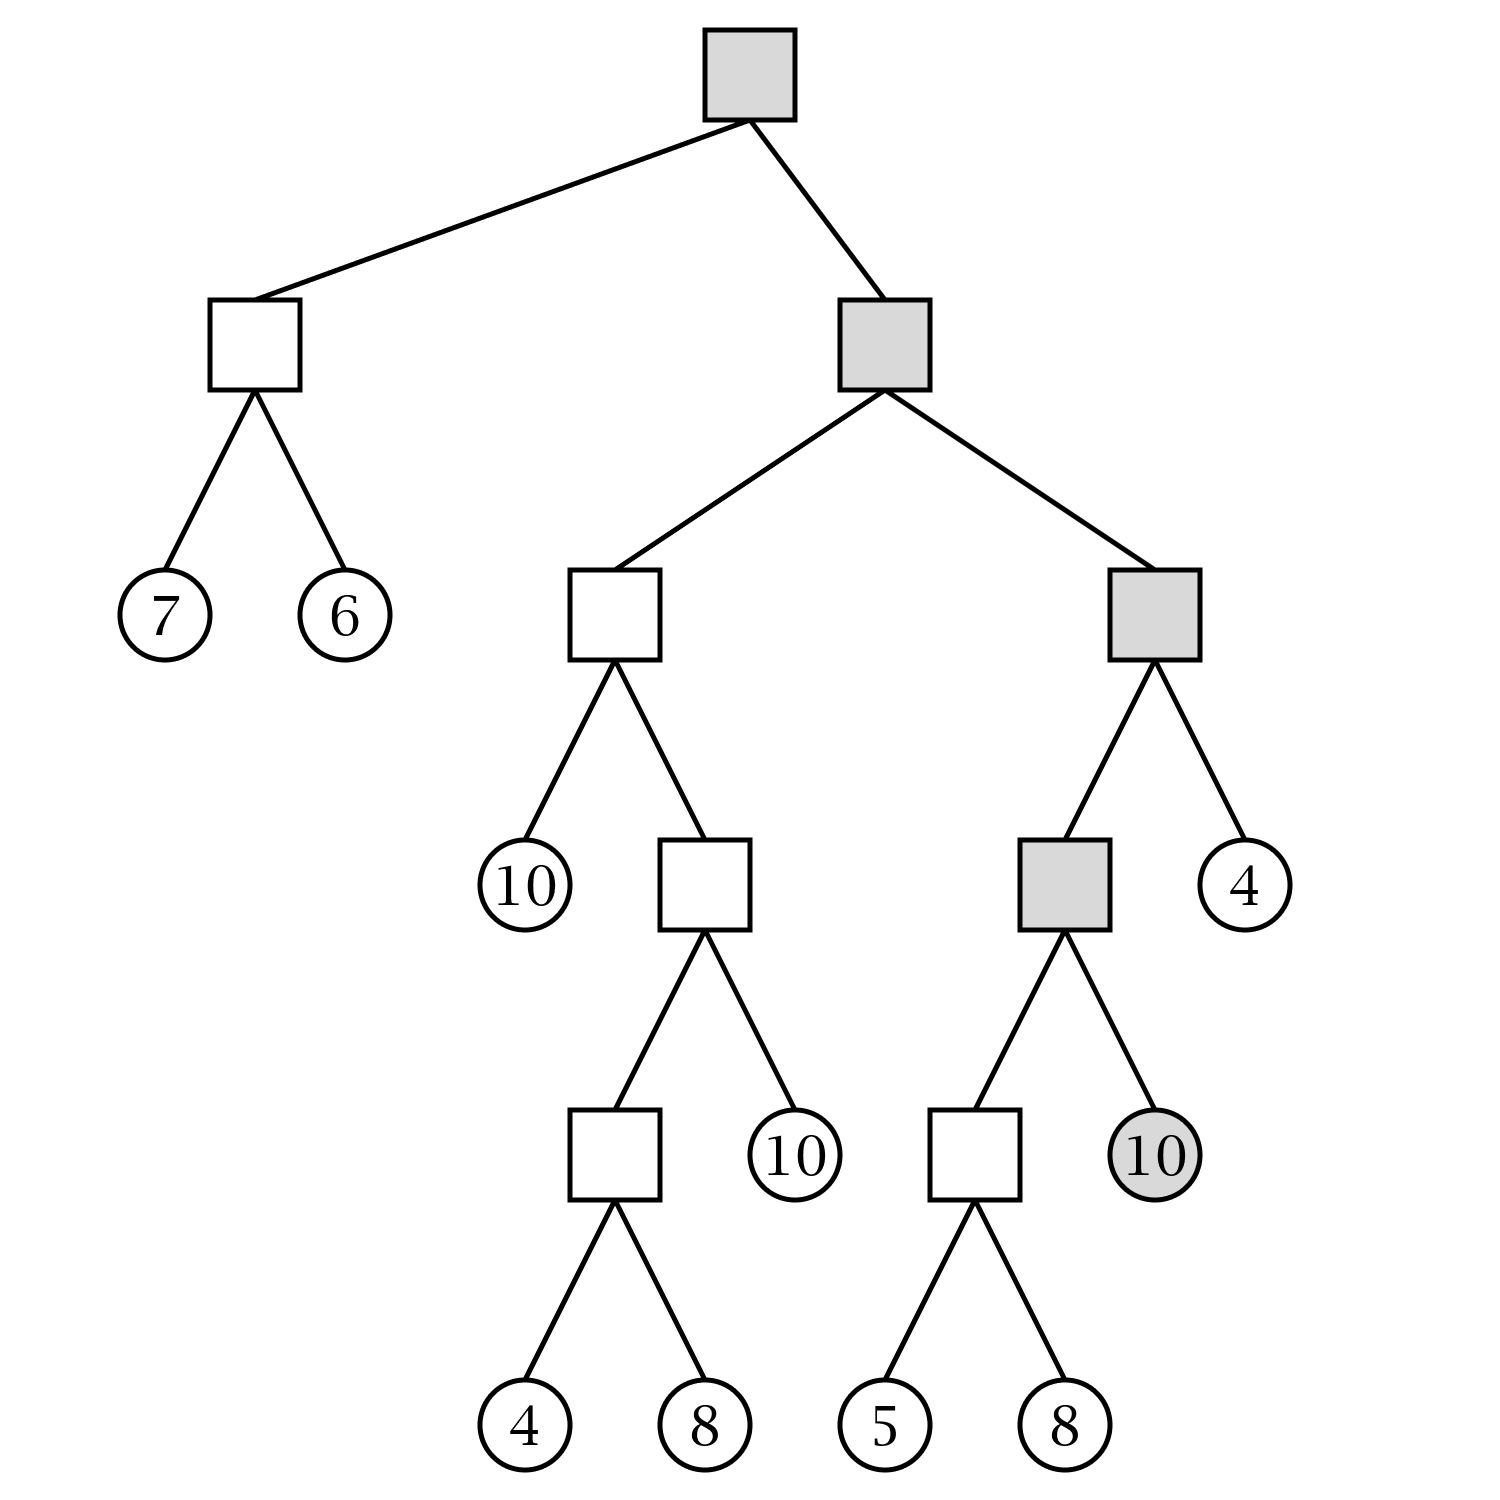
\includegraphics[width=\textwidth]{chapters/algorithms/annoy/figures/traversal-2.png}
        \caption{Binary tree corresponding to the second partitioning.}
        \label{fig:annoy-7-d}
    \end{subfigure}
    
    \caption{Two trees in the Annoy forest. Each tree is generated independently with a random set of splits.}
    \label{fig:annoy-7}
\end{figure}

\noindent
Since each tree contains all points, some points may appear in multiple leaf nodes across different trees. The union of these leaf nodes identifies candidate points that are likely to include the nearest neighbors (Figure~\ref{fig:annoy-8-a}).

Distances from the query point to these candidate points are computed during the simultaneous traversal of all trees, with a single priority queue prioritizing nodes and facilitating retrieval of the top $n$ nearest neighbors (Figure~\ref{fig:annoy-8-b}).

\begin{figure}[H]
    \centering
    \begin{subfigure}[t]{0.48\textwidth}
        \centering
        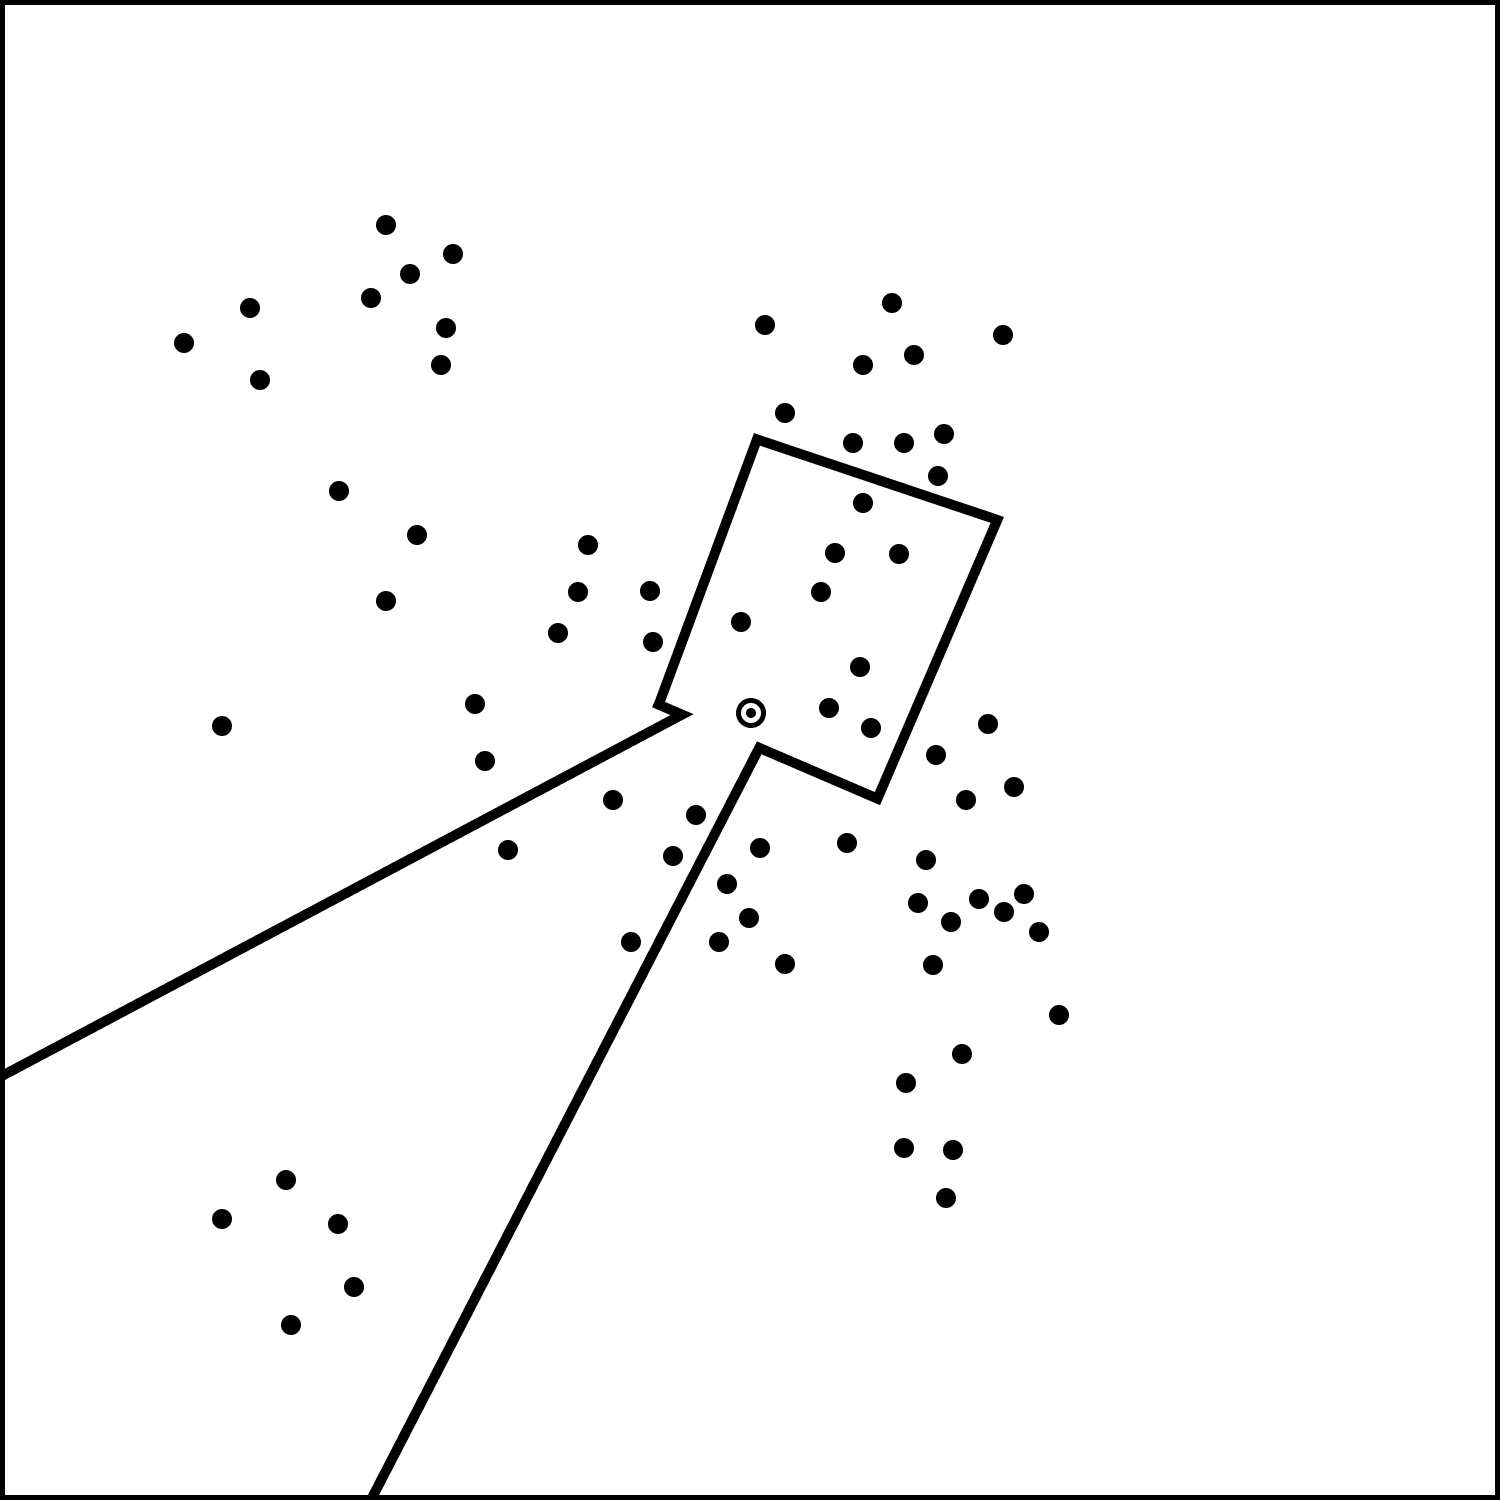
\includegraphics[width=\textwidth]{chapters/algorithms/annoy/figures/union.png}
        \caption{Union of leaf nodes containing the query point across multiple trees in the forest.}
        \label{fig:annoy-8-a}
    \end{subfigure}
    \hfill
    \begin{subfigure}[t]{0.48\textwidth}
        \centering
        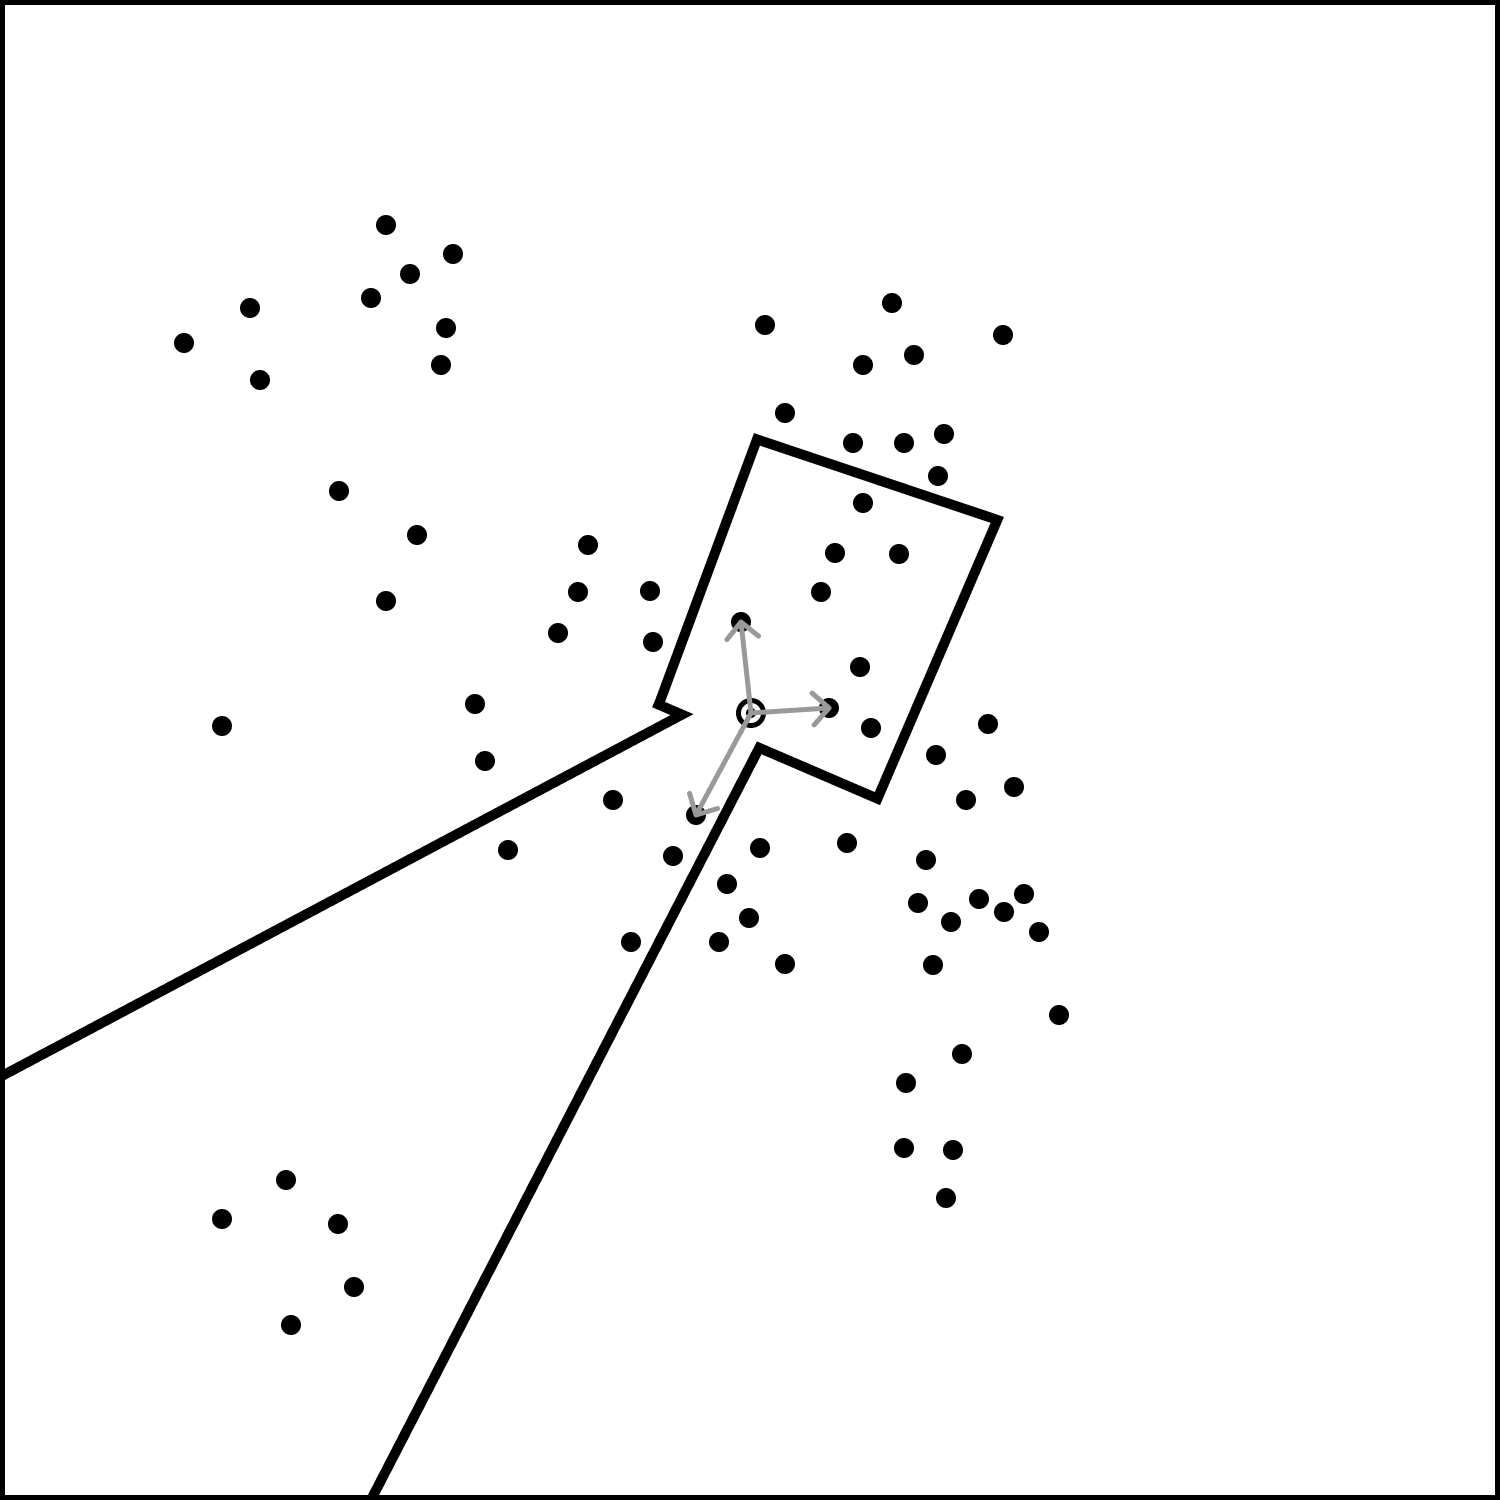
\includegraphics[width=\textwidth]{chapters/algorithms/annoy/figures/distances.png}
        \caption{Distances from the query point to the closest points.}
        \label{fig:annoy-8-b}
    \end{subfigure}
    \caption{Candidate points and distance evaluation during Annoy forest search.}
    \label{fig:annoy-8}
\end{figure}

\noindent
Increasing the number of trees generally improves recall by providing more opportunities to encounter favorable splits. The practical upper limit is typically constrained by available memory resources.

\subsection{Analysis of Annoy}

\subsubsection{Parameters}

There are two main parameters that control the performance of Annoy: the number of trees $n\_trees$ and the number of nodes inspected during query execution $search\_k$ \cite{spotify-annoy}.

\paragraph{$n\_trees$ Parameter}

The parameter $n\_trees$ defines the number of trees in the Annoy forest and is set at build time. Increasing $n\_trees$ generally improves recall, since more independent random partitions raise the chance of obtaining favorable splits. This improvement, however, comes at the cost of longer index construction and increased memory usage. In practice, the value of $n\_trees$ is typically chosen as large as possible within available memory limits \cite{spotify-annoy}.

\paragraph{$search\_k$ Parameter}

The parameter $search\_k$ specifies the number of nodes inspected during query execution and is set at runtime. Larger values improve recall by considering more candidate points, but also increase query latency. If not explicitly specified, $search\_k$ defaults to $n \times n\_trees$, with $n$ denoting the number of requested nearest neighbors. In practice, $search\_k$ is usually set as large as possible given the time constraints for query processing \cite{spotify-annoy}.

\subsubsection{Multiple Processes and Memory Sharing}

A distinctive feature of Annoy is its ability to share a single index across multiple processes. This is achieved by creating static file-based indexes that can be memory-mapped (mmap) by any number of processes. By decoupling index creation from loading, the same index file can be distributed or passed around, allowing immediate lookups without rebuilding the structure.

This approach is particularly useful in high-performance or distributed environments, where multiple CPUs or workers need to access the index concurrently. Only a single copy of the index needs to be built, minimizing both construction overhead and memory usage. Moreover, because index creation is separate from lookup, no additional vectors can be added once the index is built \cite{spotify-annoy}.